\section{Pilot Study}

% To understand how language boundary affect cooperative game experience, we recruit 9 Taiwaneses and 3 Japaneses and divided into 2 separate group-types(i)Taiwan-Taiwan, (ii)Taiwan-Japan. We have validated that Taiwanese players don’t understand Japanese and vise versa. We choose three different cooperative games on Steam[1] (so that player can talk to each other through Steam Talk), Rocketbirds:Hardboiled Chicken(Cooperative Action Game) ,Portal 2 (Cooperative Puzzle Game), Monaco (Cooperative Stealth Game).To emulate quick match via Internet, two players are playing these games at two distinct rooms using headphones for communication. Players play these three games 30 minutes for each. After playing each game, players will fill up an eSFQ[2] questionnaire for rapid assessment of game experiences and conduct an open-ended interviews.

In order to understand how language boundary affect cooperative game experience, we proceeded pilot study, added a factor of language boundary, for players to play the famous cooperative game on the market today. We recruited players with 9 Taiwaneses and 3 Japanese, and we divided them into 2 separated group-types: (i)Taiwan-Taiwan, (ii)Taiwan-Japan. We had confirmed that all Taiwanese players don't understand Japanese and vice versa. We chose three different famous cooperative games: Rocketbirds:Hardboiled Chicken (Cooperative Action Game), Portal 2 (Cooperative Puzzle Game), Monaco (Cooperative Stealth Game). In addition, all three games were chosen from Steam\cite{PS1} so that players can talk to each other through Steam Talk. Besides, in order to emulate quick match via Internet, both players were placed at two different rooms and used headphones to communicate with each other. Each time players proceed these three games for 30 minutes. Last but not least, players had to fill up an eSFQ\cite{eSFQ} questionnaire after playing each game respectively, and we also conducted an open-ended interviews to understand game experience. 

\begin{table}[!h]
% \renewcommand\arraystretch{1.2}
  \centering
  \begin{tabular}{
  !{\vrule width2pt}c
  !{\vrule width2pt}p{0.7\columnwidth}
  !{\vrule width2pt}}
    \Xhline{2px}
    \tabhead{Game} &
    \multicolumn{1}{p{0.7\columnwidth}!{\vrule width2pt}}{\centering\tabhead{User Feedback from T-J group}\\} \\
    \Xhline{2px}
    Rocket Birds & 
    \begin{itemize}
	\item Although language boundary make more times 
    to finish the game, but challenges still can 
    be beated with patience.
    \item We can't communicate through language, but the game also offer few ways to communicate like move and jump.
    \item We can't discuss who has to change position and how to defense.
	\end{itemize}
    \\
    \Xhline{2px}
    Portal 2 & 
    \begin{itemize}
    \item It’s hard to explain my solution to solve puzzles. I am tired to communicate.
    \item You need to cooperate indeedly but it's really hard if you can't talk.
    \item I don't understand what my partner's thought. I can only guess it by his movement.
    \end{itemize}
    \\
    \Xhline{2px}
    Monaco & 
    \begin{itemize}
    \item I want my partner to lure the guardian, and he doesn't understand it. But I can still complete my mission with other approach.
    \item This game is simple. We don't really need any communication with each other.
    \item The game doesn't really need any sort of co-op behavior.
    \end{itemize}
    \\
    \Xhline{2px}
  \end{tabular}
  \caption{User Feedback from T-J group}
  \label{tab:table1}
\end{table}

\begin{figure}[!h]
\centering
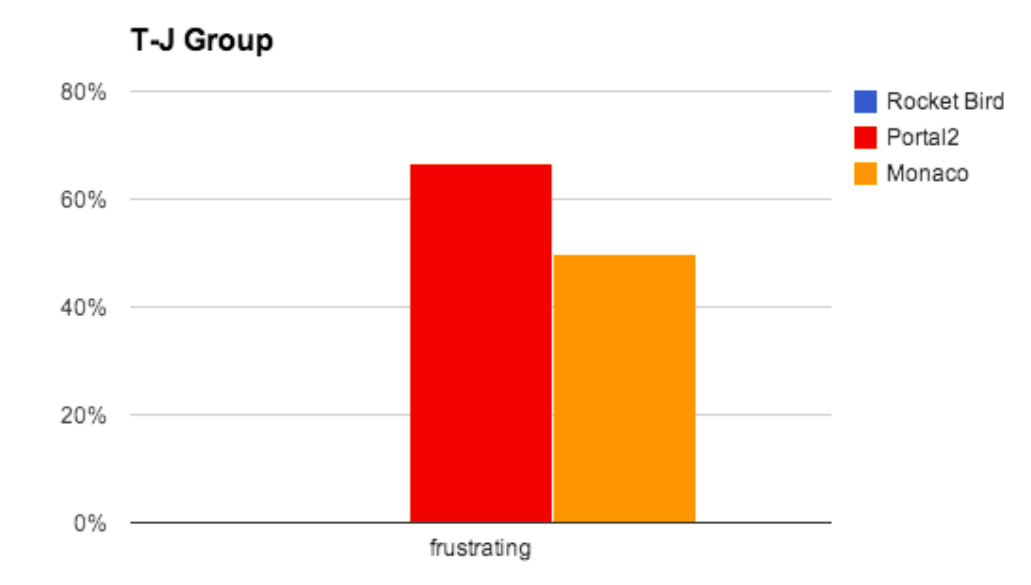
\includegraphics[width=0.9\columnwidth]{Figures/PS_F1.png}
\caption{Frustrating index of eSFQ}
\label{fig:figure1}
\end{figure}


\subsection{Result}

Hi, I'm result!!! :)


\subsection{Discussion}
\subsubsection{Rocket Birds}
% According to our pilot study result, There is language boundary issue while playing Rocket Chicken,but it doesn’t cause frustrating and affect game experience significantly. We think this is because there are no complex concept to transmit. The main gameplay is dodging and shooting, players don’t need high-level-feature communication in this game.

After our pilot study, the result shows that language boundary has an impact while playing Rocket Birds, but it doesn't cause frustrated and doesn't significantly affect game experience. After our discussion, we consider that the reason to lead to this result is because no complex concept needs to be tranmitted during the game. The main gameplay is dodging and shooting, players don't need high-level-feature communication in this game.


\subsubsection{Portal 2}
% Portal2 is reported the most frustrating while playing with different language players. Interview shows that language boundary really obstruct the process of gameplay and causing frustrating. We think it is because that,the main gameplay in portal 2 is solving complex puzzles, and it is impossible to pass the level with only one player, high-level-feature communication is required ,but it is hard to accomplish while playing with different language speaker.

Portal 2 is reported as the most frustrated gameplay experience while playing with different language players. From our interview record, it shows that language boundary really obstructs the process of gameplay between players and causes frustrated. To explain this condition, we think the reason is that the main gameplay in Portal 2 is to solve complex puzzles, which leads to pass the level with only one player is almost impossible. As a result, high-level-feature communication is required for playing Portal 2. However, it is hard to accomplish the game while playing with different language speaker.


\subsubsection{Monaco}
% Monaco is reported not cooperative at all and highly frustrated. In our observation, T-J group player only try to communicate at first and give up communicating really quickly, because this game is not restrict to single solution and forcing player to cooperate together. Even though two players are not cooperative working, single player can still stealth in the building and finish his mission, but the difficulty will significantly increase. We think this cause the game frustrating and players think this game is not cooperative at all.

The third game, Monaco, is reported not cooperative at all and frustrated while playing the game. In our observation, T-J group player only try to communicate at first, and then give up to communicate with each other quickly. The reason is that Monaco is not restrict to single solution to the problem and force players to cooperate together. Under this gameplay environment, single player can still finish his own mission secretly in the building, even though both players are not cooperative working and then difficulty will increase significantly. We consider that this situation would make gameplay experience be frustrated and players would think this game does not need to cooperate at all.

\begin{table}[!h]
\renewcommand\arraystretch{1.5}
  \centering
  \begin{tabular}{
  !{\vrule width2pt}p{0.2\columnwidth}
  !{\vrule width2pt}p{0.4\columnwidth}
  !{\vrule width2pt}p{0.4\columnwidth}
  !{\vrule width2pt}}
    \Xhline{2px}
    \tabhead{} &
    \multicolumn{1}{p{0.4\columnwidth}!{\vrule width2pt}}{\centering\tabhead{Cooperative Only}} &
    \multicolumn{1}{p{0.4\columnwidth}!{\vrule width2pt}}{\centering\tabhead{Non-Cooperative Allowed}} \\
    \Xhline{2px}
    High-Level Feature Communication & 
    Portal 2:\newline 
    Keep trying to communicate.\newline
    Tiring on hard communicate.\newline
    Frustrated Experience. & 
    Monaco:\newline 
    Give up communicate.\newline
    Play like single player game.\newline
    Frustrated Experience. \\
    \Xhline{2px}
    Low-Level Feature Communication & 
    \multicolumn{2}{c!{\vrule width2pt}}
    {
    Rocket Birds:\newline
    Not Affect Game Experience.
    }
    \\
    \Xhline{2px}
  \end{tabular}
  \caption{Observation from Pilot Study}
  \label{tab:table2}
\end{table}



